% *******************************************************************************
% * Copyright (c) 2007 by Elexis
% * All rights reserved. This document and the accompanying materials
% * are made available under the terms of the Eclipse Public License v1.0
% * which accompanies this distribution, and is available at
% * http://www.eclipse.org/legal/epl-v10.html
% *
% *  $Id: abrechnung.tex 2470 2007-06-03 07:01:57Z rgw_ch $
%
%*******************************************************************************
% !Mode:: "TeX:UTF-8" (encoding info for WinEdt)

\section{Abrechnungsbezogene Views}
\subsection{Konsultationen nach Datum}
%\begin{floatingfigure}[l] {70mm}
\begin{figure}[hb]
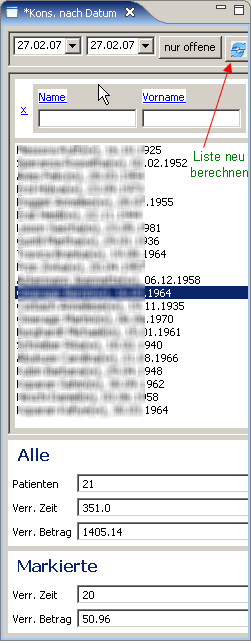
\includegraphics{images/konnd}
\caption{Konsultation nach Datum}
\label{fig:konnd}
%\end{floatingfigure}
\end{figure}
Diese View (s. Abb. \ref{fig:konnd}) dient dazu, Ihnen alle in einem bestimmten
Zeitraum stattgefundenen
Konsultationen aufzulisten. Sie können in den Datumsfeldern oben das Start- und
das Enddatum des gewünschten Zeitraums angeben.

Der Knopf \glqq nur offene\grqq kann betätigt werden, um in die Auflistung nur
solche Konsultationen aufzunehmen, für die noch keine Rechnung erstellt wurde.

Wenn Sie die Daten oder den Auswahlknopf geändert haben, erscheint die neu
berechnete Liste erst nach Klick auf den Button \glqq Liste neu berechnen\grqq.

Im unteren Abschnitt der View sehen Sie die Gesamtzahl der Konsultationen im
gewählten Zeitraum, sowie die (vom Abrechnungssystem her vorgegebene)
verrechnete Zeit und den verrechneten Betrag. Im Feld darunter sehen Sie
dieselben Angaben für die aktuell markierte Konsultation.

Sie können diese View also auch verwenden, um Abends kurz die Konsultationen des Tages
durchzugehen um unverrechnete oder falsch verrechnete zu korrigieren. Die Liste
kann auch zur einfacheren Lesbarkeit ausgedruckt werden (\textsc{ViewMenu-Liste drucken})
\subsection{Konsultationen zum Verrechnen}
\index{Abrechnung} Diese View (s. fig. \ref{fig:konsv}) dient dazu, diejenigen
Konsultationen
auszuwählen, von welchen eine Rechnung erstellt werden soll. Es werden dabei nur
die Konsultationen des aktuellen Mandanten angezeigt.
\begin{figure}[hb]
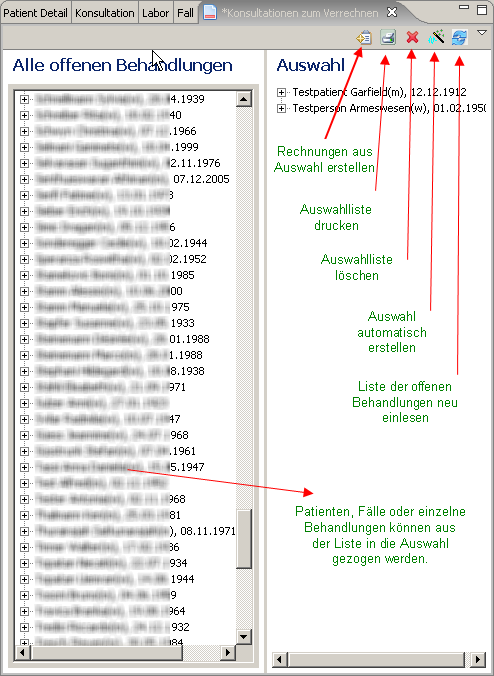
\includegraphics{images/konsv}
\caption{Konsultation zur Verrechnung auswählen}
\label {fig:konsv}
\end{figure}
Hierzu gibt es folgende Möglichkeiten:
\begin{itemize}
  \item Automatische Auswahl: Dabei werden die Konsultationen nach einem
  bestimmten Algorithmus automatisch ausgewählt und in die Auswahlliste
  übertragen.
  \item Patientennamen aus der Liste in die Auswahl ziehen: Dadurch werden alle
  Konsultationen aller Fälle des gewählten Patienten zur Abrechnung markiert.
  \item Fälle aus der Liste in die Auswahl ziehen: Dadurch werden alle
  Konsultationen der gewählten Fälle zur Abrechnung markiert.
  \item Konsultationen aus der Liste in die Auswahl ziehen: Dadurch werden nur
  die gewählten Konsultationen zur Abrechnung vorgemerkt.
\end{itemize}
Bei allen Methoden können Sie die Auswahl nachträglich noch beliebig ändern. Sie
können weitere Elemente zufügen, oder Sie können (nach Rechtsklick auf ein
Element in der Auswahl) Elemente entfernen, oder Sie können die ganze Auswahl
wieder löschen. Zu diesem Zeitpunkt sind noch keinerlei Änderungen der Daten
erfolgt.

Wenn Sie die Auswahl fertig erstellt haben, können Sie auf \glqq Rechnungen
erstellen\grqq klicken, dann werden Rechnungen für alle in der Auswahl
befindlichen Elemente erstellt. Dabei werden immer alle Konsultationen, die zu
einem Fall gehören, zusammengefasst. Wenn von einem Patienten also mehrere Fälle
in der Auswahl sind, werden auch mehrere Rechnungen erstellt.

\subsection{Konto}
\index{Konto}In dieser View sehen Sie alle Kontobewegungen eines bestimmten Patienten.
Rechnungen werden als negative, Zahlungen und Storno als positive
Buchungen erfasst, so dass Sie einfach über mehrere Rechnungen und Zahlungen
hinweg erkennen können, wo Sie finanziell mit dem betreffenden Klienten stehen.

\subsection{Konto-Liste}
Diese Liste zeigt alle Kontobewegungen insgesamt an.

\subsection{Leistungen}


\subsection{Rechnungen}

